\usetikzlibrary {automata,positioning}
% "(CDE|(BC)+)|A"
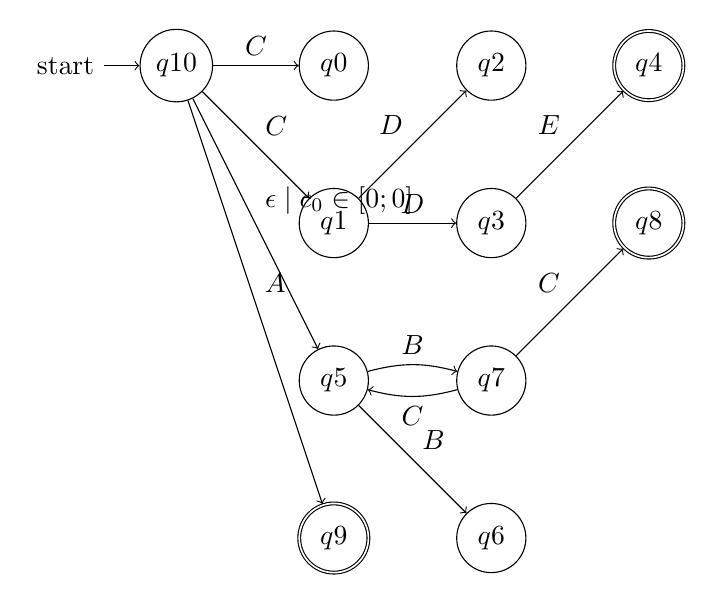
\begin{tikzpicture}[auto]
    \node[state] at (2, 0)(q0){$q0$};
    \node[state] at (2, -2)(q1){$q1$};
    \node[state] at (4, 0)(q2){$q2$};
    \node[state] at (4, -2)(q3){$q3$};
    \node[state, accepting] at (6, 0)(q4){$q4$};
    \node[state] at (2, -4)(q5){$q5$};
    \node[state] at (4, -6)(q6){$q6$};
    \node[state] at (4, -4)(q7){$q7$};
    \node[state, accepting] at (6, -2)(q8){$q8$};
    \node[state, accepting] at (2, -6)(q9){$q9$};
    \node[state, initial] at (0, 0)(q10){$q10$};

    \path[->]
    (q1)edge node{$D$}(q2)
    (q3)edge node{$E$}(q4)
    (q1)edge node{$D$}(q3)
    (q5)edge node{$B$}(q6)
    (q7)edge node{$C$}(q8)
    (q5)edge [bend left=15] node{$B$}(q7)
    (q7)edge [bend left=15] node{$C$}(q5)
    (q10)edge node{$C$}(q0)
    (q10)edge node{$C$}(q1)
    (q10)edge node{$\epsilon\mid c_0\in[0;0]$}(q5)
    (q10)edge node{$A$}(q9)
    ;
\end{tikzpicture}
\captionof{figure}{Graph layout with all pruning disabled.}
\label{fig:nopruning}